\chapter{Specifikacija programske potpore}
		
	\section{Funkcionalni zahtjevi}
			
			
			\noindent \textbf{Dionici:}
			
			\begin{packed_enum}
				
				\item Voditelj postaje
				\item Istraživač	
				\item Tragač
				\item Administrator
				\item Neregistrirani korisnik
				\item Razvojni tim
				
				
			\end{packed_enum}
			
			\noindent \textbf{Aktori i njihovi funkcionalni zahtjevi:}
			
			
			\begin{packed_enum}
				\item  \underbar{Voditelj postaje može:}
				
				\begin{packed_enum}
					
					\item vidjeti kartu s ponuđenim postajama
					\item odabrati postaju čiji voditelj želi postati
					\item odabrati tragače svoje postaje
					\item definirati način prijevoza svojih tragača - pješke, dronom, automobilom, cross motorom, brodom ili helikopterom
					\item prihvatiti ili odbiti zahtjev za tragačima od istraživača
					
				\end{packed_enum}
			
				\item  \underbar{Istraživač može:}
				
				\begin{packed_enum}
					
					\item kreirati nove akcije pretraživanja i praćenja životinja
					\item poslati zahtjev za tragačima voditelju postaje
					\item podijeliti zadatke tragačima koje je dobio od voditelja postaje
					\item vidjeti interaktivnu kartu s podacima o pozicijama životinja, tragača i postaja
					\item odabrati kriterije filtriranja karte
					\item ostaviti komentar tragačima na akciji
					
				\end{packed_enum}
			
				\vspace{36pt}
				
				\item  \underbar{Tragač može:}
				
				\begin{packed_enum}
					
					\item na karti vidjeti svoje zadatke, životinje te ostale tragače na istoj akciji
					\item Obavljati zadatke koje mu je dodijelio istraživač
					\item Prilikom obavljanja akcije ostaviti komentar za ostale tragače
					
				\end{packed_enum}
				
				\item  \underbar{Administrator može:}
				
				\begin{packed_enum}
					
					\item Pregledati popis svih registriranih korisnika i njihovih podataka
					\item Mijenjati osobne podatke i dodijeljena prava svim korisnicima
					\item Potvrditi ili odbiti registraciju istraživača i voditelja postaje
					
				\end{packed_enum}
				
				\item  \underbar{Neregistrirani korisnik može:}
				
				\begin{packed_enum}
					
					\item Poslati zahtjev za registraciju
				
				\end{packed_enum}
				
				
			\end{packed_enum}
			
			\eject 
			
			
				
			\subsection{Obrasci uporabe}
				
				
				\subsubsection{Opis obrazaca uporabe}
				
					

					\noindent \underbar{\textbf{UC1 - Registracija}}
					\begin{packed_item}
	
						\item \textbf{Glavni sudionik: }Neregistrirani korisnik
						\item  \textbf{Cilj:} Stvoriti korisnički račun za pristup sustavu
						\item  \textbf{Sudionici:} Baza podataka
						\item  \textbf{Preduvjet:} -
						\item  \textbf{Opis osnovnog tijeka:}
						
						\item[] \begin{packed_enum}
	
							\item Korisnik odabire opciju za registraciju
							\item Korisnik popunjava korisničke podatke
							\item Korisnik prima e-mail za verifikaciju korisničkog računa
						\end{packed_enum}
						
						\item  \textbf{Opis mogućih odstupanja:}
						
						\item[] \begin{packed_item}
	
							\item[2.a] Odabir već zauzetog korisničkog imena ili e-mail adrese, unos podataka
							u pogrešnom formatu, nepotpun unos podataka
							\item[] \begin{packed_enum}
								
								\item Sustav obavještava korisnika o neuspjeloj registraciji i upućuje na pogrešna polja
								\item Korisnik mijenja ili nadopunjava potrebne podatke te završava unos ili odustaje od registracije
								
							\end{packed_enum}
							
						\end{packed_item}
					\end{packed_item}
					
					\noindent \underbar{\textbf{UC2 - Prijava u sustav}}
					\begin{packed_item}
						
						\item \textbf{Glavni sudionik: }Korisnik, administrator
						\item  \textbf{Cilj:} Dobiti pristup korisničkom sučelju
						\item  \textbf{Sudionici:} Baza podataka
						\item  \textbf{Preduvjet:} Potvrđena registracija
						\item  \textbf{Opis osnovnog tijeka:}
						
						\item[] \begin{packed_enum}
							
							\item Unos korisničkog imena i lozinke
							\item Potvrda o ispravnosti unesenih podataka
							\item Pristup korisničkom sučelju

						\end{packed_enum}
						
						\item  \textbf{Opis mogućih odstupanja:}
						
						\item[] \begin{packed_item}
							
							\item[2.a] Neispravno korisničko ime ili lozinka
							\item[] \begin{packed_enum}

								\item Sustav obavještava korisnika o neispravnom unosu podataka i traži korisnika da ponovi unos ili da se registrira
								\item Korisnik unosi ispravne podatke te završava unos ili odustaje od prijave
								
							\end{packed_enum}
							
						\end{packed_item}
					\end{packed_item}
					
					\noindent \underbar{\textbf{UC3 - Pregled osobnih podataka}}
					\begin{packed_item}
						
						\item \textbf{Glavni sudionik: }Korisnik
						\item  \textbf{Cilj:} Pregledati osobne podatke
						\item  \textbf{Sudionici:} Baza podataka
						\item  \textbf{Preduvjet:} Korisnik je prijavljen
						\item  \textbf{Opis osnovnog tijeka:}
						
						\item[] \begin{packed_enum}
							
							\item Korisnik odabire opciju ”Prikaz osobnih podataka”
							\item Sustav prikazuje osobne podatke korisnika
						\end{packed_enum}

					\end{packed_item}
					
					\noindent \underbar{\textbf{UC4 - Promjena osobnih podataka}}
					\begin{packed_item}
						
						\item \textbf{Glavni sudionik: }Korisnik
						\item  \textbf{Cilj:} Promijeniti osobne podatke
						\item  \textbf{Sudionici:} Baza podataka
						\item  \textbf{Preduvjet:} Korisnik je prijavljen
						\item  \textbf{Opis osnovnog tijeka:}
						
						\item[] \begin{packed_enum}
							
							\item Korisnik odabire opciju ”Prikaz osobnih podataka”
							\item Korisnik odabire opciju ”Ažuriraj osobne podatke”
							\item Korisnik mijenja svoje osobne podatke
							\item Korisnik sprema promjene
							\item Baza podataka se ažurira
						\end{packed_enum}
						
						\item  \textbf{Opis mogućih odstupanja:}
						
						\item[] \begin{packed_item}
							
							\item[3.a] Unos podataka u pogrešnom formatu, brisanje podataka iz obaveznih polja
							\item[] \begin{packed_enum}
								
								\item Sustav obavještava korisnika o neispravnom unosu podataka i traži korisnika da ponovi unos
								\item Korisnik unosi ispravne podatke ili odustaje od izmjena
								
							\end{packed_enum}
							
						\end{packed_item}
					\end{packed_item}
					
					\noindent \underbar{\textbf{UC5 - Brisanje korisničkog računa}}
					\begin{packed_item}
						
						\item \textbf{Glavni sudionik: }Korisnik
						\item  \textbf{Cilj:} Izbrisati svoj korisnički račun
						\item  \textbf{Sudionici:} Baza podataka
						\item  \textbf{Preduvjet:} Korisnik je prijavljen
						\item  \textbf{Opis osnovnog tijeka:}
						
						\item[] \begin{packed_enum}
							
							\item Korisnik odabire opciju ”Prikaz osobnih podataka”
							\item Korisnik odabire opciju ”Izbriši korisnički račun”
							\item Korisnički račun se izbriše iz baze podataka
							\item Otvara se početna stranica
						\end{packed_enum}

					\end{packed_item}
					
					\noindent \underbar{\textbf{UC6 - Potvrda korisnika mailom}}
					\begin{packed_item}
						
						\item \textbf{Glavni sudionik: }Korisnik
						\item  \textbf{Cilj:} Potvrditi korisnički račun e-mailom
						\item  \textbf{Sudionici:} Baza podataka
						\item  \textbf{Preduvjet:} Korisnik je upisao podatke potrebne za registraciju
						\item  \textbf{Opis osnovnog tijeka:}
						
						\item[] \begin{packed_enum}
							
							\item Korisnik prima e-mail za verifikaciju korisničkog računa
							\item Korisnik otvara primljeni e-mail i klikne na link u poruci
							\item Link ga vodi na ekran s porukom o uspješnosti registracije
							\item Podaci o korisniku se spremaju u bazu podataka registriranih korisnika
							\item Korisnik se može prijaviti u sustav sa izabranim korisničkim imenom i lozinkom
						\end{packed_enum}
						
						\item  \textbf{Opis mogućih odstupanja:}
						
						\item[] \begin{packed_item}
							
							\item[1.a] Korisnik nije dobio e-mail zbog serverske pogreške
							\item[] \begin{packed_enum}
								
								\item Korisnik klikne na opciju ponovno pošalji e-mail
								
							\end{packed_enum}
							\item[1.b] Korisnik nije dobio e-mail zbog unosa krive e-mail adrese
								\item[] \begin{packed_enum}
								
								\item Korisnik klikne na opciju za ponovno unošenje e-mail adrese
								\item Korisnik unosi novu e-mail adresu
								
							\end{packed_enum}
							
						\end{packed_item}
					\end{packed_item}
					
					\noindent \underbar{\textbf{UC7 - Potvrda uloge od strane administratora}}
					\begin{packed_item}
						
						\item \textbf{Glavni sudionik: }Administrator
						\item  \textbf{Cilj:} Potvrditi registraciju voditelja postaje ili istraživača
						\item  \textbf{Sudionici:} Istraživač, voditelj postaje, baza podataka
						\item  \textbf{Preduvjet:} Istraživač ili voditelj su unijeli svoje podatke za registraciju
						\item  \textbf{Opis osnovnog tijeka:}
						
						\item[] \begin{packed_enum}
							
							\item Administrator se prijavljuje u sustav
							\item Administrator vidi popis neriješenih registracija
							\item Administrator otvara jednu od registracija i pregleda
							\item Administrator prihvati ili odbije registraciju
							\item Istraživač ili voditelj dobiju obavijest o prihvaćenoj/odbijenoj registraciji
						\end{packed_enum}
						
					\end{packed_item}
					\vspace{12pt}
					\vspace{12pt}
					\vspace{12pt}
					\vspace{12pt}
					\vspace{12pt}
					
					\noindent \underbar{\textbf{UC8 - Prikazivanje pozicije životinje}}
					\begin{packed_item}
						
						\item \textbf{Glavni sudionici: }Administrator, istraživač i tragač
						\item  \textbf{Cilj:} Prikaz pozicije životinje na karti
						\item  \textbf{Sudionici:} Baza podataka
						\item  \textbf{Preduvjet:} Postoji barem jedna životinja s GPS uređajem
						\item  \textbf{Opis osnovnog tijeka:}
						
						\item[] \begin{packed_enum}
							
							\item Svakih 5 sekundi se šalje lokacija životinje i sprema u bazu
							\item Prikaz karte sa lokacijama životinja u bazi
							\item Lokacija se prikazuje u obliku geom. dužine, širine i timestampa
							\item Mogućnost filtriranja karte po vrsti životinje
						\end{packed_enum}
						
					\end{packed_item}
					
					\noindent \underbar{\textbf{UC9 - Prikazivanje pozicije tragača}}
					\begin{packed_item}
						
						\item \textbf{Glavni sudionik: } Korisnik
						\item  \textbf{Cilj:} Prikaz pozicije tragača na karti
						\item  \textbf{Sudionici:} Baza podataka
						\item  \textbf{Preduvjet:} Postoji barem jedan tragač s GPS uređajem
						\item  \textbf{Opis osnovnog tijeka:}
						
						\item[] \begin{packed_enum}
							
							\item Korisnik otvara opciju "Karta"
							\item Korisnik filtrira kartu tako da pokazuje tragače
							
						\end{packed_enum}
						
					\end{packed_item}
					
					\noindent \underbar{\textbf{UC10 - Prikazivanje pozicije postaje}}
					\begin{packed_item}
						
						\item \textbf{Glavni sudionik: } Korisnik
						\item  \textbf{Cilj:} Na karti pokazati geografsku poziciju postaje
						\item  \textbf{Sudionici:} Baza podataka
						\item  \textbf{Preduvjet:} Postoji barem jedna postaja
						\item  \textbf{Opis osnovnog tijeka:}
						
						\item[] \begin{packed_enum}
							
							\item Korisnik odabire opciju "Postaje"
							\item Aplikacija pokazuje kartu sa svim postajama
							\item Korisnik u polje predodređeno za tekst upisuje ime postaje čiju geografsku poziciju želi detaljnije pogledati
						\end{packed_enum}
						
					\end{packed_item}
					
					\noindent \underbar{\textbf{UC11 - Prikaz informacija o životinji}}
					\begin{packed_item}
						
						\item \textbf{Glavni sudionik: }Istraživač, tragač
						\item  \textbf{Cilj:} Prikaz informacija o pojedinoj životinji (povijest kretanja i trenutna lokacija, opis jedinke, slika i naziv vrste)
						\item  \textbf{Sudionici:} Baza podataka
						\item  \textbf{Preduvjet:} -
						\item  \textbf{Opis osnovnog tijeka:}
						
						\item[] \begin{packed_enum}
							
							\item Istraživaču/tragaču su na karti prikazane GPS lokacije životinja
							\item Istraživač/tragač klikne na određenu životinju/GPS lokaciju 
							\item Otvaraju se podaci o životinji
						\end{packed_enum}
						
					\end{packed_item}
					
					\noindent \underline{\textbf{UC12 - Odabir postaje}}
					\begin{packed_item}
						\item \textbf{Glavni sudionik:} Voditelj
						\item \textbf{Cilj:} Odabir slobodne postaje
						\item \textbf{Sudionici:} Baza podataka
						\item \textbf{Preduvjet:} Voditelj je registriran i potvrđen
						\item \textbf{Opis osnovnog tijeka:}
						\begin{packed_enum}
							\item Nakon registracije voditelju se prikazuje karta na kojoj su označene postaje bez voditelja
							\item Voditelj proizvoljno bira postaju
							\item Promjene se spremaju u bazu
						\end{packed_enum}
						\item \textbf{Opis mogućih odstupanja:}
						\begin{packed_item}
							\item[2.a] Sve postaje već imaju voditelja 
							\begin{packed_enum}
								\item Voditelj mora pričekati da neka postaja ostane bez voditelja ili da se nova postaja otvori
							\end{packed_enum}
							\item[2.b] Odabrana postaja nije slobodna
							\begin{packed_enum}
								\item Voditelj bira neku drugu postaju
							\end{packed_enum}
						\end{packed_item}
					\end{packed_item}
					
					
					\noindent \underbar{\textbf{UC13 -Definiranje kompetencija tragača}}
					\begin{packed_item}
						
						\item \textbf{Glavni sudionik: } Voditelj
						\item  \textbf{Cilj:} Odabir tragača unutar jedne postaje te definiranje kompetencija pojedinog tragača
						\item  \textbf{Sudionici:} Baza podataka, tragač
						\item  \textbf{Preduvjet:} Voditelj je odabrao postaju
						\item  \textbf{Opis osnovnog tijeka:}
						
						\item[] \begin{packed_enum}
							
							\item Nakon odabira postaje voditelju se prikazuje popis svih tragača koji nisu raspoređeni ni u jednoj postaji
							\item Voditelj klikom odabire tragače i njihove kompetencije
							\item Tragaču i u bazi se ažuriraju promjene
						\end{packed_enum}
						
						\item  \textbf{Opis mogućih odstupanja:}
						
						\item[] \begin{packed_item}
							
							\item[1.a] Ne postoji slobodan tragač 
							\item[] \begin{packed_enum}
								
								\item  Voditelj čeka da se registrira novi tragač ili da tragač bude otpušten iz postaje kojoj je dodijeljen
								
								
							\end{packed_enum}
						
							
						\end{packed_item}
					\end{packed_item}
					
					\vspace{12pt}
					\vspace{12pt}
					\vspace{12pt}
					
					\noindent \underbar{\textbf{UC14 - Uređivanje kompetencija tragača}}
					\begin{packed_item}
						
						\item \textbf{Glavni sudionik:} Voditelj
						\item  \textbf{Cilj:} Izmjena kompetencija tragača 
						\item  \textbf{Sudionici:} Baza podataka, tragač
						\item  \textbf{Preduvjet:} Postoji barem jedan tragač u postaji voditelja
						\item  \textbf{Opis osnovnog tijeka:}
						
						\item[] \begin{packed_enum}
							
							\item Voditelj odabire jednog tragača
							\item Voditelj dodaje nove ili briše postojeće kompetencije odabranog tragača
							\item Unešene promjene se spremaju u bazu podataka
							\item Voditelju i tragaču se prikazuju ažurirane kompetencije
						\end{packed_enum}
					\end{packed_item}
					
					\noindent \underbar{\textbf{UC15 - Brisanje tragača}}
					\begin{packed_item}
						
						\item \textbf{Glavni sudionik: }Voditelj
						\item  \textbf{Cilj:} Trajno brisanje tragača iz postaje
						\item  \textbf{Sudionici:} Baza podataka, voditelj
						\item  \textbf{Preduvjet:} Tragač je dio voditeljeve postaje
						\item  \textbf{Opis osnovnog tijeka:}
						
						\item[] \begin{packed_enum}
							
							\item Voditelj odabire određenog tragača
							\item Voditelj ga briše iz svoje postaje
							\item Unešena promjena se sprema u bazu podataka
							\item Tragač dobiva informaciju o voditeljevoj odluci
							\item Tragač postaje dostupan ostalim voditeljima i može biti izabran za drugu postaju
						\end{packed_enum}
					\end{packed_item}
					
					\noindent \underbar{\textbf{UC16 - Pregled popisa tragača}}
					\begin{packed_item}
						
						\item \textbf{Glavni sudionik: }Voditelj
						\item  \textbf{Cilj:} Pregled svih tragača u njegovoj postaji
						\item  \textbf{Sudionici:} Baza podataka, voditelj
						\item  \textbf{Preduvjet:} Tragač je dio voditeljeve postaje
						\item  \textbf{Opis osnovnog tijeka:}
						
						\item[] \begin{packed_enum}
							
							\item Voditelj odabire prikaz tragača svoje postaje
							\item Voditelju se prikaže popis njegovih tragača
							\item Voditelj ima mogućnost brisati i uređivati podatke svojih tragača
						\end{packed_enum}
					\end{packed_item}
					
					\vspace{12pt}
					\vspace{12pt}
					\vspace{12pt}
					\vspace{12pt}
					\vspace{12pt}
					
					\noindent \underbar{\textbf{UC17 - Pregled zahtjeva}}
					\begin{packed_item}
						
						\item \textbf{Glavni sudionik: }Voditelj
						\item  \textbf{Cilj:} Započeti komunikaciju između voditelja i istraživača 
						\item  \textbf{Sudionici:} Voditelj, istraživač
						\item  \textbf{Preduvjet:} -
						\item  \textbf{Opis osnovnog tijeka:}
						
						\item[] \begin{packed_enum}
							
							\item Istraživač voditelju šalje zahtjev za tragačima
							\item U zahtjevu je zapisan broj potrebnih ljudi i zadaci u akciji
							\item Voditelj dobiva zahtjev
							\item Voditelj može pregledati sve svoje zahtjeve
							\item Voditelj može odabrati zahtjev koji želi obraditi
						\end{packed_enum}
					\end{packed_item}
					
					\noindent \underbar{\textbf{UC18 - Obrada zahtjeva}}
					\begin{packed_item}
						
						\item \textbf{Glavni sudionik: } Voditelj
						\item  \textbf{Cilj:} Prihvatiti/odbaciti zahtjev
						\item  \textbf{Sudionici:} Baza podataka
						\item  \textbf{Preduvjet:} Voditelj je prijavljen i poslan je barem jedan zahtjev od strane istraživača
						\item  \textbf{Opis osnovnog tijeka:}
						
						\item[] \begin{packed_enum}						
							\item Voditelj odabire opciju "Obrada zahtjeva"
							\item Voditelju se prikazuje karta na kojoj se nalaze samo tragači koji pripadaju njegovoj postaji
							\item Voditelju se prikazuje broj tragača potrebnih za akciju te popis zadataka akcije
							\item Voditelj s obzirom na zadatke odabire kvalificirane tragače  
							\item Ako ima dovoljan broj kvalificiranih tragača, voditelj šalje popis istraživaču od kojeg je dobio zahtjev, a u suprotnom odbija zahtjev
						\end{packed_enum}
					\end{packed_item}
					
					\noindent \underbar{\textbf{UC19 - Kreiranje akcije}}
					\begin{packed_item}
						
						\item \textbf{Glavni sudionik: } Istraživač
						\item  \textbf{Cilj:} Kreiranje nove akcije
						\item  \textbf{Sudionici:} Baza podataka, tragači
						\item  \textbf{Preduvjet:} Istraživač je prijavljen u sustav
						\item  \textbf{Opis osnovnog tijeka:}
						
						\item[] \begin{packed_enum}
							
							\item Istraživač odabire opciju "Nova akcija"
							\item Istraživač odabire broj tragača, potrebne kvalifikacije tragača te upisuje zadatke
						\end{packed_enum}
					\end{packed_item}
					
					\noindent \underbar{\textbf{UC20 - Slanje zahtjeva voditelju}}
					\begin{packed_item}
						
						\item \textbf{Glavni sudionik: } Istraživač, voditelj
						\item  \textbf{Cilj:} Poslati zahtjev voditelju
						\item  \textbf{Sudionici:} Baza podataka
						\item  \textbf{Preduvjet:} Istraživač je kreirao novu akciju.
						\item  \textbf{Opis osnovnog tijeka:}
						
						\item[] \begin{packed_enum}
							
							\item Istraživač šalje voditelju/voditeljima zahtjev za tragačima s napisanim zadacima
						\end{packed_enum}
					\end{packed_item}
					
					\noindent \underbar{\textbf{UC21 - Pregled stanja zahtjeva}}
					\begin{packed_item}
						
						\item \textbf{Glavni sudionik: } Istraživač
						\item  \textbf{Cilj:} Uvid u stanje zahtjeva
						\item  \textbf{Sudionici:} Baza podataka
						\item  \textbf{Preduvjet:} Istraživač je prijavljen u sustav te je poslan barem jedan zahtjev
						\item  \textbf{Opis osnovnog tijeka:}
						
						\item[] \begin{packed_enum}
							
							\item Istraživač odabire opciju "Određeni zahtjev" (npr. "Postavljanje GPS-uređaja na zeca")
							\item Istraživaču se prikazuje stanje "Određenog zahtjeva", je li zahtjev odobren, odbijen ili je u stanju čekanja 
						\end{packed_enum}
					\end{packed_item}
					
					\noindent \underbar{\textbf{UC22 - Kreiranje zadataka}}
					\begin{packed_item}
						
						\item \textbf{Glavni sudionik: }Istraživač
						\item  \textbf{Cilj:} Kreirati zadatke za tragače
						\item  \textbf{Sudionici:} Baza podataka
						\item  \textbf{Preduvjet:} Istraživač je u postupku kreiranja akcije
						\item  \textbf{Opis osnovnog tijeka:} 
						\item[] \begin{packed_enum}
							
							\item Ispod podnaslova zadaci istraživač klikne plus
							\item Istraživač definira zadatak
						\end{packed_enum}
					\end{packed_item}
					
					\vspace{36pt}
					\vspace{36pt}
					\vspace{36pt}
					\noindent \underbar{\textbf{UC23 - Dodjela zadataka}}
					\begin{packed_item}
						
						\item \textbf{Glavni sudionik: }Istraživač
						\item  \textbf{Cilj:} Dodijeliti zadatke pojedinim tragačima
						\item  \textbf{Sudionici:} Baza podataka
						\item  \textbf{Preduvjet:} Istraživač je prijavljen u sustav i voditelj je prihvatio zahtjev za akcijom
						\item  \textbf{Opis osnovnog tijeka:}
						
						\item[] \begin{packed_enum}
							
							\item Istraživaču se prikaže lista zadataka u akciji
							\item Istraživaču se prikaže lista tragača kompatibilnih za određene zadatke
							\item Istraživač odabire koji tragač će obaviti pojedine zadatke
						\end{packed_enum}
						
					\end{packed_item}
					
					\noindent \underbar{\textbf{UC24 - Definiranje prikaza na karti}}
					\begin{packed_item}
						
						\item \textbf{Glavni sudionik: }Korisnik
						\item  \textbf{Cilj:} Prikazati željene podatke na karti
						\item  \textbf{Sudionici:} Baza podataka
						\item  \textbf{Preduvjet:} Korisnik je potvrđen
						\item  \textbf{Opis osnovnog tijeka:}
						
						\item[] \begin{packed_enum}
							
							\item Korisnik odabire predmet filtracije podataka na karti
						\end{packed_enum}
						
					\end{packed_item}
					
					\noindent \underbar{\textbf{UC25 - Postavljanje komentara na karti}}
					\begin{packed_item}
						
						\item \textbf{Glavni sudionik: }Tragač, istraživač, baza podataka
						\item  \textbf{Cilj:} Informiranje i komunikacija istraživača i/ili tragača na akciji 
						\item  \textbf{Sudionici:} Istraživač, tragač
						\item  \textbf{Preduvjet:} Akcija je u tijeku 
						\item  \textbf{Opis osnovnog tijeka:}
						
						\item[] \begin{packed_enum}
							
							\item Istraživač/Tragač označava poziciju na karti 
							\item Istraživač/Tragač zapisuje komentar
						\end{packed_enum}
				
					\end{packed_item}
					
					\noindent \underbar{\textbf{UC26 - Pregled komentara}}
					\begin{packed_item}
						
						\item \textbf{Glavni sudionik: } Istraživač, tragač
						\item  \textbf{Cilj:} Pregledati komentare
						\item  \textbf{Sudionici:} Baza podataka
						\item  \textbf{Preduvjet:} Mora postojati barem jedan komentar
						\item  \textbf{Opis osnovnog tijeka:}
						
						\item[] \begin{packed_enum}
							
							\item Istraživač/Tragač filtrira kartu kako bi pokazivala komentare
							\item Odabire komentar koji želi pročitati
						\end{packed_enum}
						
						
					\end{packed_item}
					
					\noindent \underbar{\textbf{UC27 - Brisanje komentara}}
					\begin{packed_item}
						
						\item \textbf{Glavni sudionik:} Istraživač, tragač
						\item  \textbf{Cilj:} Obrisati objavljeni komentar
						\item  \textbf{Sudionici:} Baza podataka
						\item  \textbf{Preduvjet:} Postojanje komentara
						\item  \textbf{Opis osnovnog tijeka:}
						
						\item[] \begin{packed_enum}
							
							\item Glavni sudionik odabire komentar
							\item Glavni sudionik odabire opciju "Obriši komentar"
							\item Komentar se briše iz baze podataka
							\item Komentar se više ne prikazuje istraživačima i tragačima
						\end{packed_enum}
					\end{packed_item}
					
					\noindent \underbar{\textbf{UC28 - Prikaz karte s tragačima na akciji}}
					\begin{packed_item}
						
						\item \textbf{Glavni sudionik:} Korisnik
						\item  \textbf{Cilj:} Pregled lokacija tragača na karti
						\item  \textbf{Sudionici:} Baza podataka
						\item  \textbf{Preduvjet:} Prijavljen korisnik
						\item  \textbf{Opis osnovnog tijeka:}
						
						\item[] \begin{packed_enum}
							
							\item Korisnik odabire prikaz karte s tragačima
							\item Aplikacija prikazuje kartu s lokacijama tragača na akciji
						\end{packed_enum}
					\end{packed_item}
					
					\noindent \underbar{\textbf{UC29 - Pregled zadatka}}
					\begin{packed_item}
						
						\item \textbf{Glavni sudionik:} Istraživač, tragač
						\item  \textbf{Cilj:} Pregled detalja pojedinog zadatka
						\item  \textbf{Sudionici:} Baza podataka
						\item  \textbf{Preduvjet:} Istraživač je kreirao zadatak i dodijelio ga tragaču
						\item  \textbf{Opis osnovnog tijeka:}
						
						\item[] \begin{packed_enum}
							
							\item Glavni sudionik odabire zadatak
							\item Aplikacija prikazuje detalje zadatka
						\end{packed_enum}
					\end{packed_item}
					

				\subsubsection{Dijagrami obrazaca uporabe}
					
					
				
				\begin{figure}[H]
					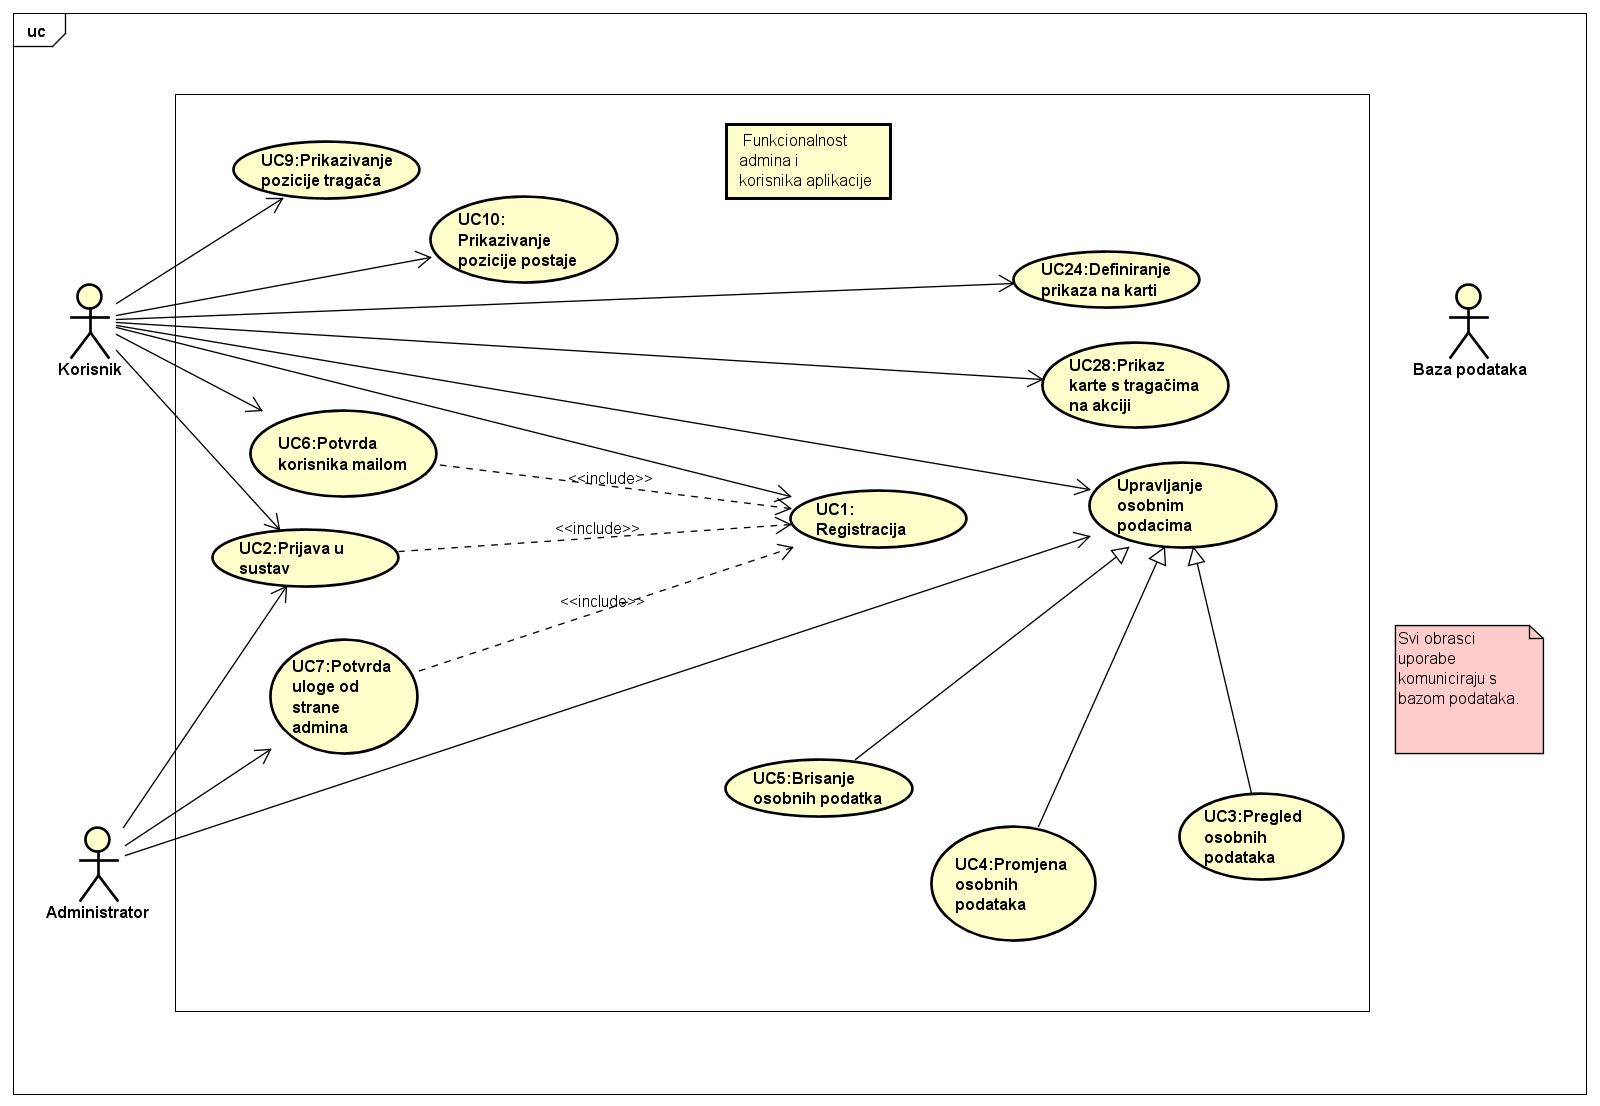
\includegraphics[width=\textwidth]{slike/Dijagram_obrasca_uporabe_funkcionalnost_admina_i_korisnika_aplikacije.PNG} %veličina u odnosu na širinu linije
					\caption{Dijagram obrasca uporabe, funkcionalnost admina i korisnika aplikacije}
					\label{fig:Dijagram_obrasca_uporabe_funkcionalnost_admina_i_korisnika_aplikacije} %label mora biti drugaciji za svaku sliku
				\end{figure}
				
				
				\begin{figure}[H]
					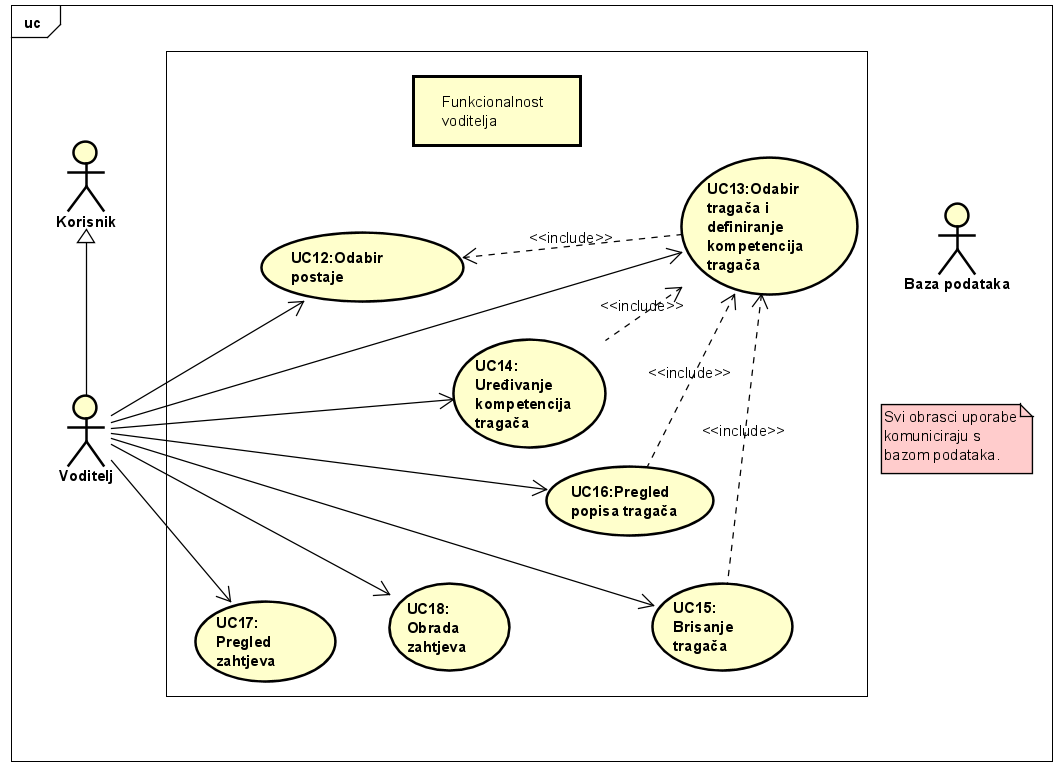
\includegraphics[width=\textwidth]{slike/Dijagram_obrasca_uporabe_funkcionalnost_voditelja.PNG} %veličina u odnosu na širinu linije
					\caption{Dijagram obrasca uporabe, funkcionalnost voditelja}
					\label{fig:Dijagram_obrasca_uporabe_funkcionalnost_voditelja} %label mora biti drugaciji za svaku sliku
				\end{figure}
				
				
				\begin{figure}[H]
					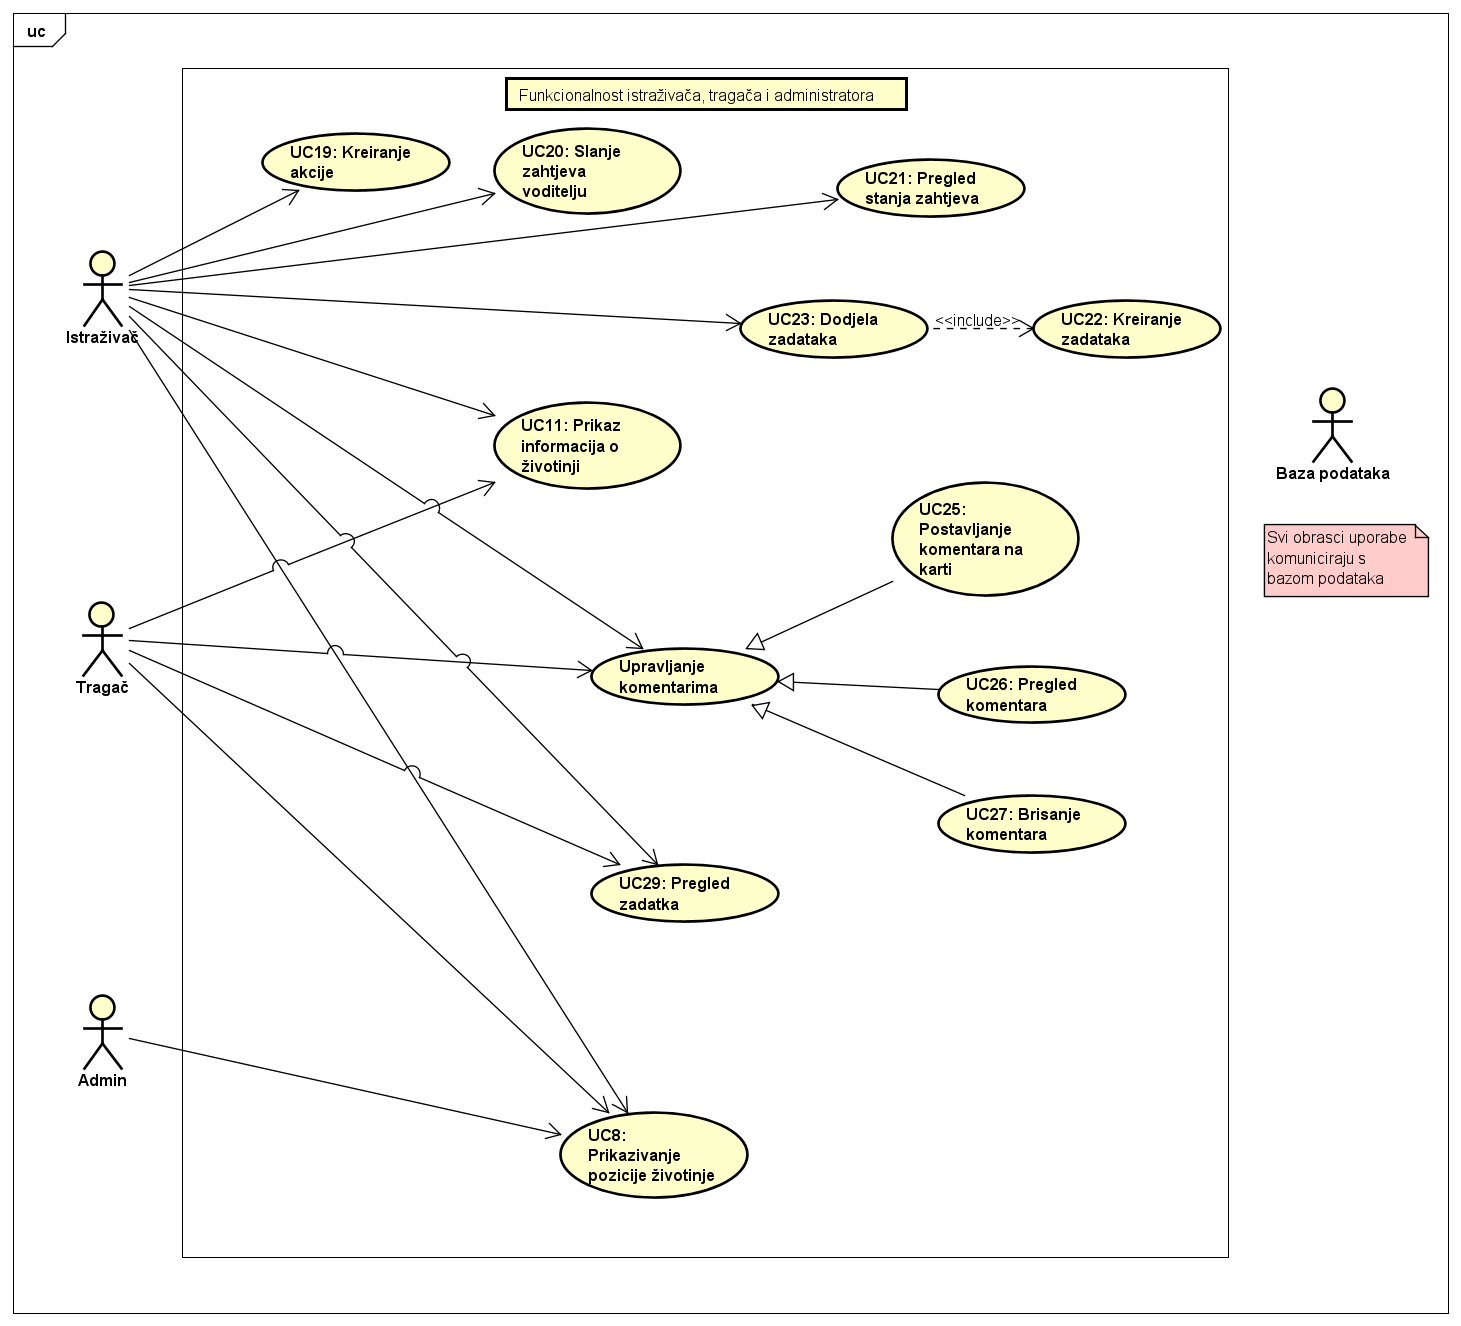
\includegraphics[width=\textwidth]{slike/Dijagram_obrasca_uporabe_funkcionalnost_istrazivaca_tragaca_i_administratora.PNG} %veličina u odnosu na širinu linije
					\caption{Dijagram obrasca uporabe, funkcionalnost istraživača i tragača }
					\label{fig:Dijagram_obrasca_uporabe_funkcionalnost_istrazivaca_tragaca_i_administratora} %label mora biti drugaciji za svaku sliku
				\end{figure}		
				
				\vspace{360pt}
				
			\subsection{Sekvencijski dijagrami}
			
				\textbf{Obrazac uporabe UC8 - Prikazivanje pozicije životinje}\\
			
				Svakih 30 sekundi spremaju se podaci o GPS uređaju životinje u bazu podataka.
				Nakon određenog vremena (npr. 30 min), web aplikacija šalje upit bazi podataka za vrijednosti koordinata. Baza podataka vraća vrijednosti koordinata web aplikaciji.  Web aplikacija uz pomoć dobivenih koordinata zabilježuje
				poziciju životinje na karti.
				\begin{figure}[H]
					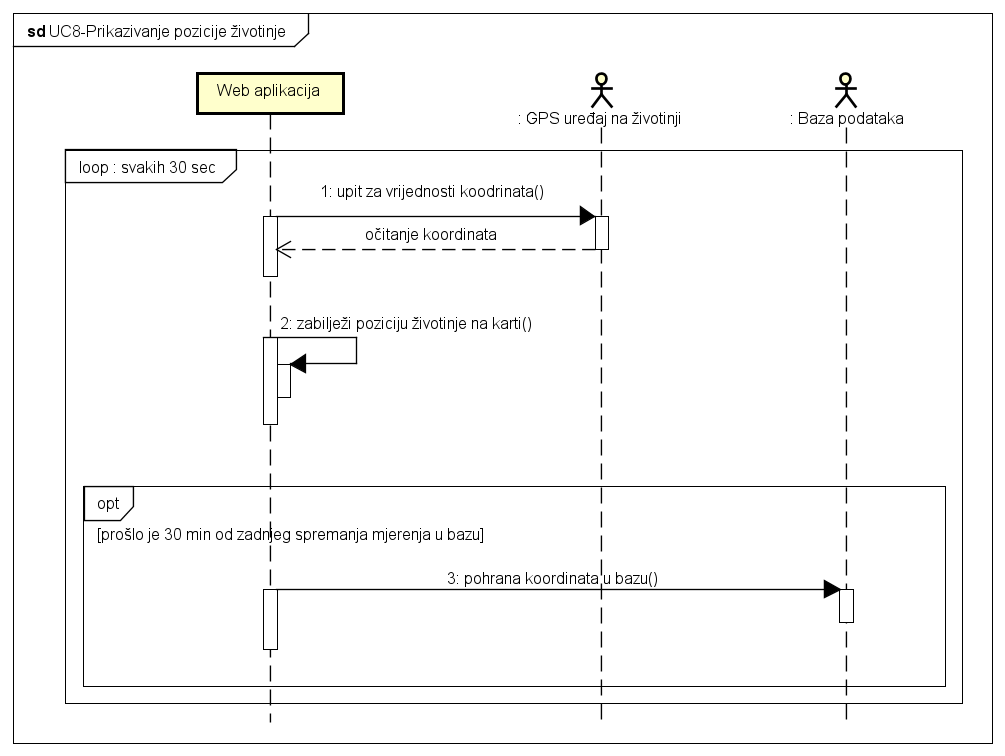
\includegraphics[width=\textwidth]{slike/UC8-PrikazivanjePozicijeZivotinje.PNG} %veličina u odnosu na širinu linije
					\caption{Sekvencijski dijagram za UC8}
					\label{fig:UC8-PrikazivanjePozicijeZivotinje} %label mora biti drugaciji za svaku sliku
				\end{figure}
				
				\vspace{60pt}
				\vspace{48pt}
				
				\textbf{Obrazac uporabe UC19-Kreiranje akcije}\\
				
				Istraživač zahtjeva kreiranje akcije te se otvara ekran za kreiranje akcije. Istraživač upisuje naslov i odabire postaju kojoj će poslati akciju iz liste postaja koju mu vraća poslužitelj. Istraživač zatražuje dodavanje zadatka te odabire koji zadatak treba obaviti iz liste koju mu vraća poslužitelj. Također, odabire kompetencije koje tragač mora imati za pripadajući zadatak iz liste koju mu vraća poslužitelj. Označuje poziciju na karti gdje treba izvršiti zadatak. Ako istraživač želi dodati detaljan opis upisuje opis u odgovarajući kvadrat. Nakon unesenih svih obveznih podataka, istraživač dodaje zadatak u akciju. Ponavlja proces dodavanja zadataka dok nije upisan željeni broj zadataka. Nakon toga poslužitelju šalje zahtjev za spremanjem akcije. Ako je zahtjev uspješno proveden poslužitelj ispisuje poruku: Akcija poslana.
				\begin{figure}[H]
					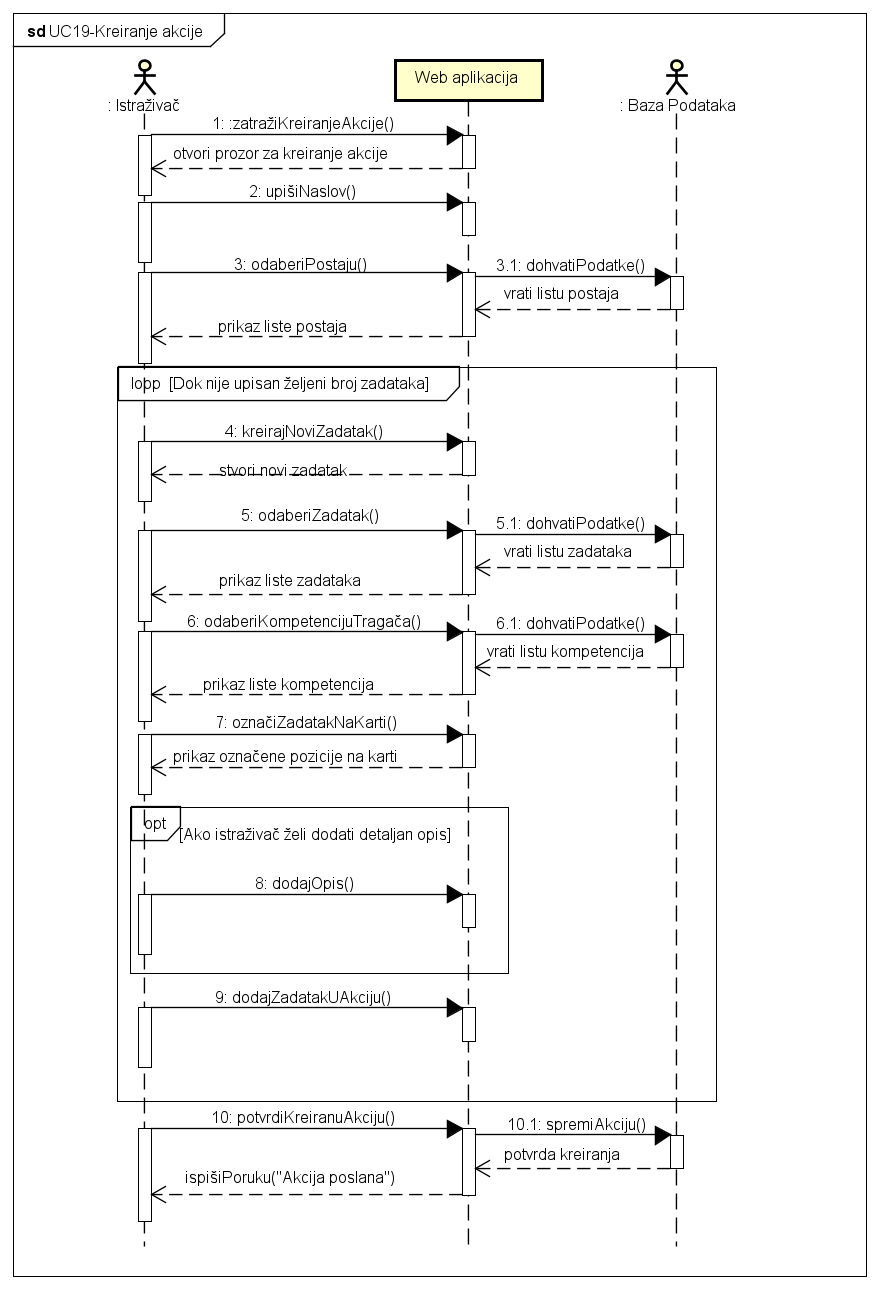
\includegraphics[width=\textwidth]{slike/UC19-KreiranjeAkcije.png} %veličina u odnosu na širinu linije
					\caption{Sekvencijski dijagram za UC19}
					\label{fig:promjene2} %label mora biti drugaciji za svaku sliku
				\end{figure}
				\eject
				
	
				\textbf{Obrazac uporabe UC25-Postavljanje komentara na karti}\\
				
				Tragač ili istraživač zatražuje dodavanje komentara na kartu te mu se omogućuje odabir pozicije na karti. Nakon što označi poziciju, upisuje komentar. Potvrđuje upis komentara čime se poslužitelju javlja da spremi komentar na zadanu poziciju. Ako je komentar uspješno spremljen, šalje poruku korisniku (tragaču ili istraživaču): Komentar dodan.
				\begin{figure}[H]
					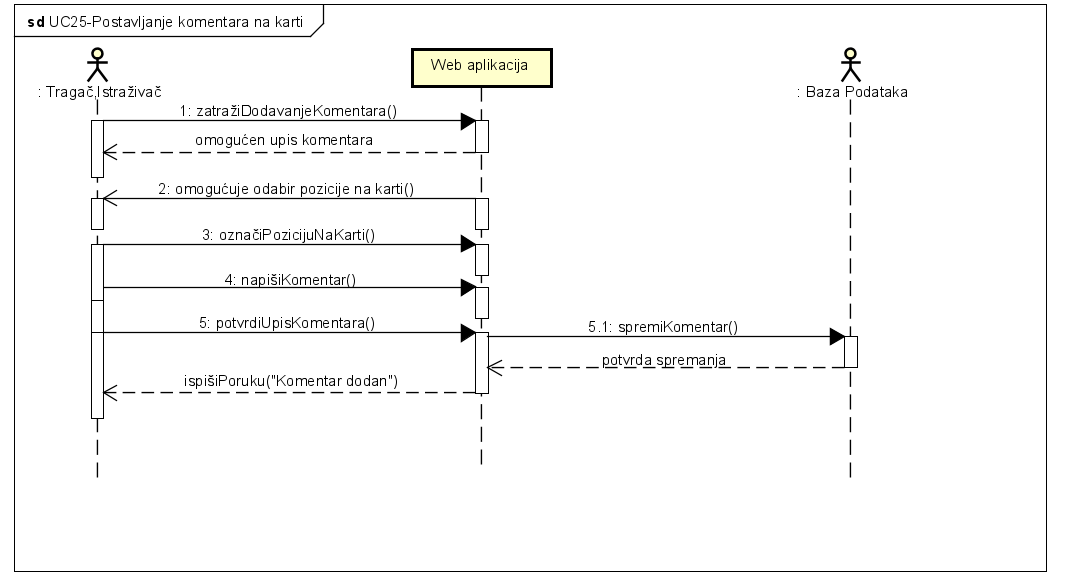
\includegraphics[width=\textwidth]{slike/UC25-PostavljanjeKomentaraNaKarti.png} %veličina u odnosu na širinu linije
					\caption{Sekvencijski dijagram za UC25}
					\label{fig:promjene2} %label mora biti drugaciji za svaku sliku
				\end{figure}
				\eject
				
				
		\section{Ostali zahtjevi}
			 
			 \begin{packed_item}
			 	\item Sustav treba omogućiti rad više korisnika u stvarnom vremenu
			 	\item Korisničko sučelje i sustav moraju podržavati hrvatsku abecedu (dijakritičke znakove) pri unosu i prikazu tekstualnog sadržaja
			 	\item Izvršavanje dijela programa u kojem se pristupa bazi podataka ne smije trajati duže od nekoliko sekundi
			 	\item Sustav treba biti implementiran kao web aplikacija koristeći objektno-orijentirane jezike
			 	\item Neispravno korištenje korisničkog sučelja ne smije narušiti funkcionalnost i rad sustava
			 	\item Sustav treba biti jednostavan za korištenje, korisnici se moraju znati koristiti sučeljem bez opširnih uputa 
			 	\item Nadogradnja sustava ne smije narušavati postojeće funkcionalnosti sustava
			 	\item Veza s bazom podataka mora biti kvalitetno zaštićena, brza i otporna na vanjske greške
			 	\item Komunikacija mora biti ostvarena sigurnim protokolom
			 	\item Pristup sustavu mora biti omogućen iz javne mreže pomoću HTTPS
			 \end{packed_item}
			 
			 
			 
	